\documentclass[12pt]{article}

\usepackage[margin=1in]{geometry}
	%changes default margins

\usepackage{setspace}
\doublespacing
	%\singlespacing,\onehalfspacing,\doublespacing can be set and everything thereafter will use that spacing. You can switch within the document as often as you wish
	
\usepackage{parskip}
%changes paragraphs to have an extra space and new indentation with paragraphs, rather than indenting every new paragraph. This is completely a stylistic choice and neither is better than the other.


\usepackage{mathtools,amssymb} %useful math stuff. there are a lot of ams* packages. If you have a math need, it's probably in there

	
	
%\usepackage{natbib}
%\usepackage{biblatex} %natbib is older and available from almost all journals, biblatex is not, but biblatex has more flexibility and options.

%\usepackage[natbib=true]{biblatex} %this often works and requires minimal changes 

%for biblatex you write \textcite{citekey} and \parencite{citekey}
%for natbib you write \citet{citekey} and \citep{citekey}. Please avoid using \cite{} since you won't control whether it's parenthetical, but you are responsible for whether you use something in text or parenthetically.
%for \usepackage[natbib=true]{biblatex} you follow the natbib style and you won't have to perform search/replaces in your document, you would only need to change the package call and bibliography call.

\usepackage{natbib}
\bibliographystyle{chicago}

%other useful packages
% \usepackage{graphicx} %for including images including pdf



\title{Project/thesis Proposal}
\author{cld4h}
\date{\today}



\begin{document}
	
	\maketitle
	
	
	\section{Introduction}
	Sentence 1 and/or 2 should very broadly describe a problem that anyone can understand. Sentence 2 or 3 should narrow down the scope of the previous sentence to something that any of the other data science students can understand. By sentence 3 or 4, you should be introducing the problem that you are going to be discussing.
	
	In a new paragraph, you'll begin talking about specifics of the problem.
	
	\section{Data Description}
	
	This section will not apply if you are primarily using a simulation study. Instead, you can describe your simulation in your methodology section. 
	\section{Literature Review}
	
	You should include relevant literature here. It should include material about other approaches that are used to solve the same problem, even if you don't plan to use those methods. It should include information about the methods you plan to use, especially if it's been used for a similar problem.
	
	\subsection{Citations}
	For citations in \LaTeX, you can use in-text citations when the citation itself is used in the sentence. Citations using \texttt{natbib} are shown here, which primarily use \texttt{citet} and \texttt{citep} commands. The same commands are used with the package call \texttt{\\usepackage[natbib=true]\{biblatex\}}\footnote{With \texttt{biblatex} (and not using \texttt{natbib=true}), the macros \texttt{citet} and \texttt{citep} are replaced by the \texttt{textcite} and \texttt{parencite}, respectively.}.
	
	If you look in the \texttt{.bib} file, there are collections of entries beginning with \texttt{\\@book,\\@article}, etc.. For example, 
	
	\begin{verbatim}
@article{lasso1996,
    Title   = {Regression shrinkage and selection via the lasso},
    Author  = {Tibshirani, Robert},
    Journal = {Journal of the Royal Statistical Society. Series B (Methodological)},
    Year    = {1996},
    Number  = {1},
    Pages   = {267--288},
    Volume  = {58}
}
	\end{verbatim}
The first thing to know is whitespace is irrelevant. You may may add/remove spaces and newlines for your convenience. You'll notice I lined up the equal signs because it's easier for me to read the text file, but the computer doesn't care; it could have all been on one long line (just like in C or Java) and it would work, though it's much more difficult to identify errors since error messages are printed corresponding to line numbers.

The second thing to know is that the entry is agnostic to citation style. You'll notice that different citation styles largely convey the same information: author, year, title, etc., but with different formats. The bib-file contains all of the information that any citation style would need and the computer formats it for that particular style. Some styles won't use all of the information in the bib-entry.

The first token always identifies the type of reference \mbox{(\texttt{\\@article})}, and then a set of braces \{...\} which identify the details of that reference. The first token in the brace must be alphanumeric and is a unique key in the bib-file for how you reference it in your text. I have chosen the key \texttt{lasso1996} because when I'm writing the article, it's easy for me to remember the lasso paper from 1996. Some people use keys in the firstauthoryear style  for consistency, and instead would call it \texttt{tibshirani96}, and if there were multiple references by the author from that year, something would need to be changed to make it unique, such as \texttt{tibshirani96a},\texttt{tibshirani96b}, etc.. If you look for bib-files through google scholar, you'll notice they often automatically include part of the title as the key. The computer does not care what you use, as long as the key is unique and matched whenever it needs to be looked up. Modern editors will auto-complete keys for you or help narrow it down by scanning your bib-file so the actual key is less important than it used to be, but in the old days, if you had to go look up what the key was, that tended to ruin your train of thought when writing so it's nice to have a convention where you can think of what the key is instantly as you're writing. People even used to be very meticulous about their bib-files by making sure it's in a particular order (e.g., chronological or alphabetical) but document searching it's not that important anymore. 

When you add a new entry to a bib-file, ensure each argument (title, author, etc.) is set equal to something either in double quotes, or in a nested set of braces (this is what I have done), followed by a comma, to delineate it from the next entry. If the right side of the equal side is a single token, like the year, it does not need quotation marks or braces, but I do it so I don't have to think about it. Very often, I find that in the format I write my bibentries, I have a missing comma at the end of a line (like at the end of Year = 1996) or I have an extra comma at the last entry (like Volume = 58,). In the first case, Year will merge with the next line and cause an error in making sense of the entry. In the second case, the extra comma at the end makes the computer assume there is more to the reference in the next line but the reference abruptly ends with the closing brace, so again it makes an error in making sense of the entry.

If you receive an error about your bib-file, it often indicates the line number in your bib file where the error was found. Very often, the error is not at that line, but a previous line or the previous entry. 

It used to be the case that you had to manually type out bib-entries. With electronic access to journals, this is largely unnecessary but with a serious caveat. If you look at the actual journal's website, there's usually a link for the plain-text bib-entry that you can copy and paste right into your bib file, and change the key to match whatever style you're using. Google scholar has a citation button in the search results that does the same thing but unfortunately, \textbf{it is often wrong or incomplete} because the automated scraping still makes mistakes. It doesn't matter what Google said the citation is, you're taking credit for the appropriate citation so you must ensure that the citation is correct, and as complete as possible. Always check the bib-entry has filled in the fields appropriately. E.g., ``et al." does not belong in the author list, you must list all the authors and leave it to the citation style to decide when ``et al." needs to be used. Always put in complete first and last names, not initials. Ensure that the actual article title and journal name is correct. There are many errors I've seen in the citations generated by Google, so thoroughly check it every time.




Your bib-file can be hundreds or thousands of references, but only the references you actually use in your \textbf{.tex} file will actually end up in your bibliography so you do not really need a separate custom bib file for each document you have. I often keep one at the root of my cloud accounts like dropbox or onedrive account and relatively reference it as \texttt{../../references.bib} if I'm only a couple folders deep. I personally have a single bib-file since I was in grad school and just keep adding to it as I need it since I often re-cite lots of the same works. 



\subsection{Citing in the \TeX\ file}
\subsubsection{Creating a bibliography}
At the location where you want the bibliography to be, put the macro 	\texttt{\\bibliography\{referencebib-file\}}. You may include relative references such as \texttt{\\bibliography\{../referencebib-file\}} but do not include the extension of .bib when using natbib, as it's assumed. Using biblatex, you must include the extension (which allows you to change it to .txt or anything else).

The macro, by default,  creates a new unnumbered section heading called `References'. However, you may change the title to `Bibliography' or something else, if you'd like, add section numbers, etc., by overriding the default. I will not get into that here but you can do an internet search: it's been asked a lot. Some answers will use pure \TeX, some answers will simply load a package that includes that \TeX code and you simply call a macro from it. The latter is the preferred approach.  

\subsubsection{Making references to the bibliography}
There are two methods of citation in your document: in-text citations and parenthetical citations. When the citation is actually a subject or object of your sentence, you use the in-text citation, like below. 	
\begin{quotation}
	\begin{verbatim}
		I will compare the results from those in \citet{lasso1996}.
	\end{verbatim}
\end{quotation}
yields the result

\begin{quotation}
	I will compare the results from those in \citet{lasso1996}.
\end{quotation}
	 
	 
	 
Use parenthetical citations to implicitly but not directly reference a fact, quote, opinion, etc.. The citation will not be a part of the sentence and is entirely parenthetical. 
	 
\begin{quotation}
	\begin{verbatim}
		This method performs well with large sample sizes \citep{hastie01}.
	\end{verbatim}
\end{quotation}
	yields the result

\begin{quotation}
		This method performs well with large sample sizes \citep{hastie01}.
\end{quotation}

The above works for citations that include author names, like author-year citations common in Statistics and many of the Social Sciences. Some citation styles, namely numeric ones common in Computer Science, IEEE, etc., may only include a number such as

\begin{quotation}
	This method performs well with large sample sizes [3].
\end{quotation}


This may effectively require that you to avoid writing sentences where the citation is used in-text and only use citations parenthetically. If you were to use \texttt{citet}, it may simply output the same as \texttt{citep} to avoid giving you an error but the sentence would look odd. I'd recommend knowing ahead of time whether your style will permit in-text citations or not. It's common that to have to re-write sentences if you wrote an article for one journal, have it rejected, and then have to rewrite the sentences for another journal that uses a different citation style. It's not hard, but takes a bit of time and care since being lazy about it results in grammatically incorrect sentences. You are responsible for ensuring that the citations are grammatically appropriate for the style you use.

\subsection {Figures}

\begin{center}
\begin{figure}
	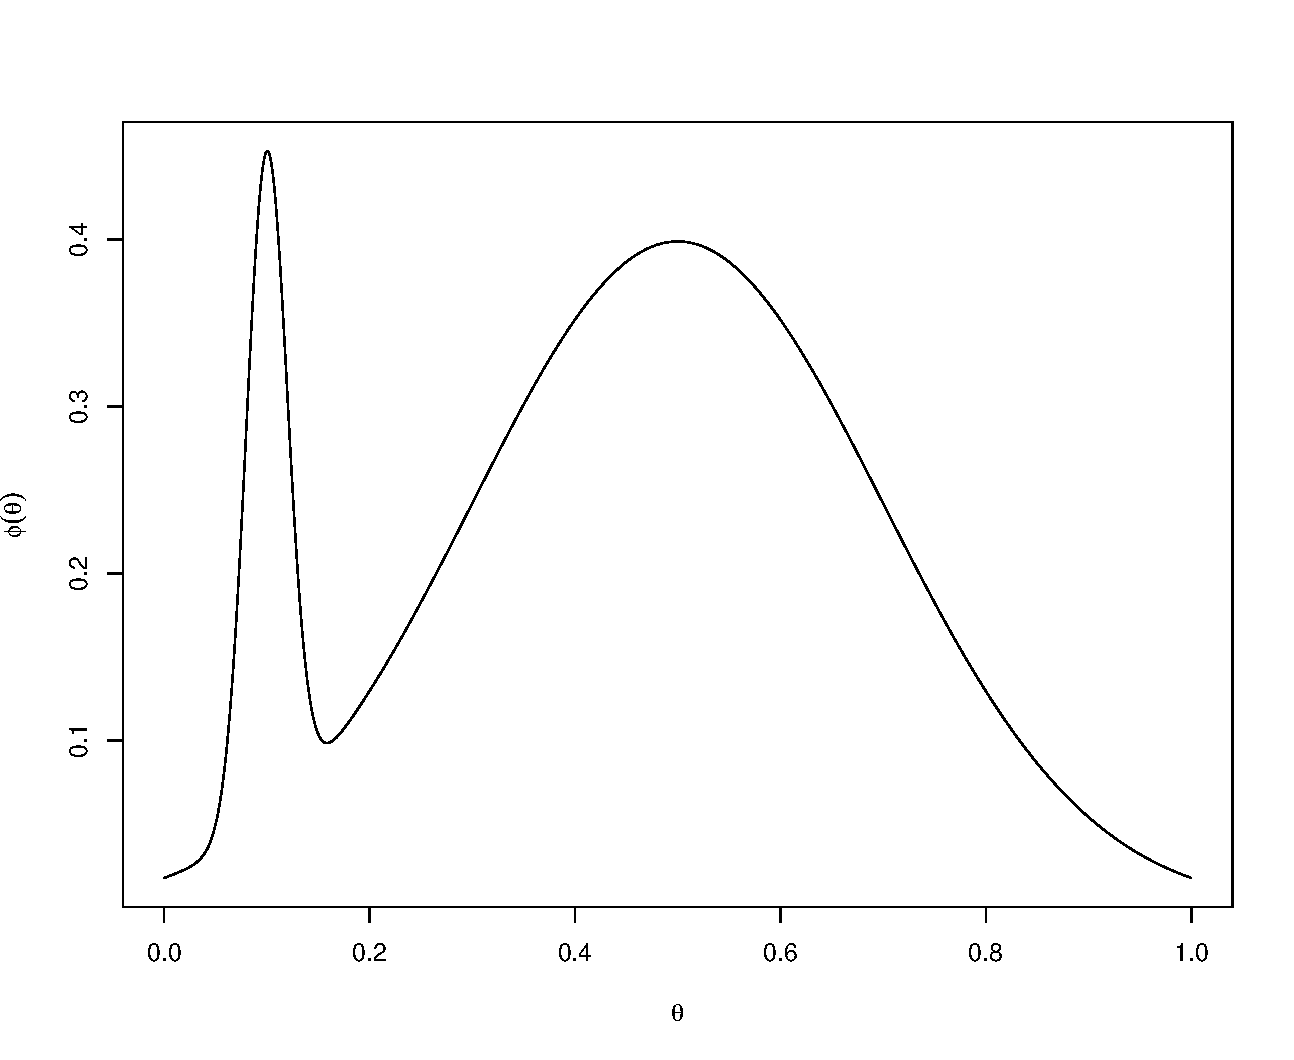
\includegraphics[width=0.9\textwidth]{Rplot}
	\caption{\label{fig:sampleimage1} This is a sample image put into a Figure. Captions should go under figures. Usually Figures are for images/visuals.}
\end{figure}
\end{center}

I can reference a particular image, such as Figure \ref{fig:sampleimage1}, using the \verb|\ref| macro. The \texttt{fig:} part is part of the key, and optional. It's often useful to use `\texttt{fig:}' for figures, `\texttt{tab:}' for Tables, `\texttt{eqn:}' or `\texttt{eq:}' for equations, etc.. as each type has its own numbering. If you have a multi-panel figure, you can make separate images and use a package that handles multiple figures. Typically, the subfigures are enumerated alphabetically and either share a caption, which individually refers to them, or each subfigure has its own caption with an overarching caption for everything. Each figure (and subfigure) can have its own \texttt{label} so you can refer to them specifically.


\subsection {Tables}
	 
\begin{table}
	\centering
		\caption{\label{tab:sampletable1} This is an example a table. The \{table\} environment makes it float like a figure, but the table itself is created in the tabular environment.  }
	\begin{tabular}{|c| c|}
		\hline
		header 1 & header 2 \\
		\hline
		$x_1$ & $y1$\\
		\hline
	\end{tabular}
\end{table}
Tables can also be included in your latex, like Table \ref{tab:sampletable1}. The text may not always match where the table is, but if it's labelled, it's easy to find. Floating objects are usually at the top or bottom of the current, previous, or next page. Where it ends up depends on typsetting rules on where it looks best, that you don't have to worry about: they have been programmed into the computer.

	\section{Methodology}
	This section should \emph{not introduce} anything new (that should have been done in the previous section). Instead, you can reference material from that section or recite the citation. 
	\section{Timeline}
	\begin{tabular}{r p{0.9\textwidth}}
		Oct 01:& \emph{-Progress form}\\
		Nov 15:& implementation complete\\
		Dec 01:& \emph{-Progress form}\\
  		Jan 10:& [Thesis only] Meeting with supervisor to create timeline for defence, (e.g., minimum 3 months before anticipated defence date, when first draft to supervisor, final draft to external/university no later than 1.5 months before defence, etc.).\\
		Jan 15:& first complete draft\\
		Feb 01:& \emph{-Progress form}\\
		Feb 15:& second draft\\
		Mar 01:& \emph{-Progress form}\\
		Mar 15:& last day to submit final draft to circulate to committee/second reader\\
		Apr 15:& presentation/defence (determined by coordinator)\\
	\end{tabular}

Thesis students should also budget thesis supervisory  meetings once a term at a time convenient for all members. E.g., end of the first month of a term (Sept 30 and Jan 30).
	\section{Supervisory Dissolution}
	The student agrees that supervision will be dissolved if any of the following happen:
	\begin{itemize}
	\item Two consecutive progress reports are unacceptable
	\item Three consecutive progress reports are concerning/unacceptable
	\item An academic integrity violation is suspected by the supervisor and suspected by at least one other faculty member.
	\end{itemize}
	
	\section{Outcomes and attribution}
	
	
		
	\bibliography{referencebibfile}
	
\end{document}

